
Um pequeno extra que permite criar um ambiente à volta do mundo, no nosso caso, acrescentar um céu ao mundo. SkyBox consiste em desenhar um cubo centrado no player cujas faces estejam no limiar da visão do mesmo, e por dentro colocar uma textura, por face, onde os lados se completem.

\-

\begin{figure}[h]
\begin{center}
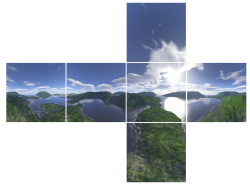
\includegraphics[width=0.5\textwidth]{images/skybox.png}
\caption{Exemplo de um textura para skybox.}
\end{center}
\end{figure}